\documentclass[11pt]{article}

    \usepackage[breakable]{tcolorbox}
    \usepackage{parskip} % Stop auto-indenting (to mimic markdown behaviour)
\usepackage{fontspec} % loaded by polyglossia, but included here for transparency 
\usepackage{polyglossia}
\setmainlanguage{russian} 
\setotherlanguage{english}
\newfontfamily\russianfont[Script=Cyrillic]{Arial}
    

    % Basic figure setup, for now with no caption control since it's done
    % automatically by Pandoc (which extracts ![](path) syntax from Markdown).
    \usepackage{graphicx}
    % Maintain compatibility with old templates. Remove in nbconvert 6.0
    \let\Oldincludegraphics\includegraphics
    % Ensure that by default, figures have no caption (until we provide a
    % proper Figure object with a Caption API and a way to capture that
    % in the conversion process - todo).
    \usepackage{caption}
    \DeclareCaptionFormat{nocaption}{}
    \captionsetup{format=nocaption,aboveskip=0pt,belowskip=0pt}

    \usepackage{float}
    \floatplacement{figure}{H} % forces figures to be placed at the correct location
    \usepackage{xcolor} % Allow colors to be defined
    \usepackage{enumerate} % Needed for markdown enumerations to work
    \usepackage{geometry} % Used to adjust the document margins
    \usepackage{amsmath} % Equations
    \usepackage{amssymb} % Equations
    \usepackage{textcomp} % defines textquotesingle
    % Hack from http://tex.stackexchange.com/a/47451/13684:
    \AtBeginDocument{%
        \def\PYZsq{\textquotesingle}% Upright quotes in Pygmentized code
    }
    \usepackage{upquote} % Upright quotes for verbatim code
    \usepackage{eurosym} % defines \euro

    \usepackage{iftex}
    \ifPDFTeX
        \usepackage[T1]{fontenc}
        \IfFileExists{alphabeta.sty}{
              \usepackage{alphabeta}
          }{
              \usepackage[mathletters]{ucs}
              \usepackage[utf8x]{inputenc}
          }
    \else
        \usepackage{fontspec}
        \usepackage{unicode-math}
    \fi

    \usepackage{fancyvrb} % verbatim replacement that allows latex
    \usepackage{grffile} % extends the file name processing of package graphics
                         % to support a larger range
    \makeatletter % fix for old versions of grffile with XeLaTeX
    \@ifpackagelater{grffile}{2019/11/01}
    {
      % Do nothing on new versions
    }
    {
      \def\Gread@@xetex#1{%
        \IfFileExists{"\Gin@base".bb}%
        {\Gread@eps{\Gin@base.bb}}%
        {\Gread@@xetex@aux#1}%
      }
    }
    \makeatother
    \usepackage[Export]{adjustbox} % Used to constrain images to a maximum size
    \adjustboxset{max size={0.9\linewidth}{0.9\paperheight}}

    % The hyperref package gives us a pdf with properly built
    % internal navigation ('pdf bookmarks' for the table of contents,
    % internal cross-reference links, web links for URLs, etc.)
    \usepackage{hyperref}
    % The default LaTeX title has an obnoxious amount of whitespace. By default,
    % titling removes some of it. It also provides customization options.
    \usepackage{titling}
    \usepackage{longtable} % longtable support required by pandoc >1.10
    \usepackage{booktabs}  % table support for pandoc > 1.12.2
    \usepackage{array}     % table support for pandoc >= 2.11.3
    \usepackage{calc}      % table minipage width calculation for pandoc >= 2.11.1
    \usepackage[inline]{enumitem} % IRkernel/repr support (it uses the enumerate* environment)
    \usepackage[normalem]{ulem} % ulem is needed to support strikethroughs (\sout)
                                % normalem makes italics be italics, not underlines
    \usepackage{soul}      % strikethrough (\st) support for pandoc >= 3.0.0
    \usepackage{mathrsfs}
    

    
    % Colors for the hyperref package
    \definecolor{urlcolor}{rgb}{0,.145,.698}
    \definecolor{linkcolor}{rgb}{.71,0.21,0.01}
    \definecolor{citecolor}{rgb}{.12,.54,.11}

    % ANSI colors
    \definecolor{ansi-black}{HTML}{3E424D}
    \definecolor{ansi-black-intense}{HTML}{282C36}
    \definecolor{ansi-red}{HTML}{E75C58}
    \definecolor{ansi-red-intense}{HTML}{B22B31}
    \definecolor{ansi-green}{HTML}{00A250}
    \definecolor{ansi-green-intense}{HTML}{007427}
    \definecolor{ansi-yellow}{HTML}{DDB62B}
    \definecolor{ansi-yellow-intense}{HTML}{B27D12}
    \definecolor{ansi-blue}{HTML}{208FFB}
    \definecolor{ansi-blue-intense}{HTML}{0065CA}
    \definecolor{ansi-magenta}{HTML}{D160C4}
    \definecolor{ansi-magenta-intense}{HTML}{A03196}
    \definecolor{ansi-cyan}{HTML}{60C6C8}
    \definecolor{ansi-cyan-intense}{HTML}{258F8F}
    \definecolor{ansi-white}{HTML}{C5C1B4}
    \definecolor{ansi-white-intense}{HTML}{A1A6B2}
    \definecolor{ansi-default-inverse-fg}{HTML}{FFFFFF}
    \definecolor{ansi-default-inverse-bg}{HTML}{000000}

    % common color for the border for error outputs.
    \definecolor{outerrorbackground}{HTML}{FFDFDF}

    % commands and environments needed by pandoc snippets
    % extracted from the output of `pandoc -s`
    \providecommand{\tightlist}{%
      \setlength{\itemsep}{0pt}\setlength{\parskip}{0pt}}
    \DefineVerbatimEnvironment{Highlighting}{Verbatim}{commandchars=\\\{\}}
    % Add ',fontsize=\small' for more characters per line
    \newenvironment{Shaded}{}{}
    \newcommand{\KeywordTok}[1]{\textcolor[rgb]{0.00,0.44,0.13}{\textbf{{#1}}}}
    \newcommand{\DataTypeTok}[1]{\textcolor[rgb]{0.56,0.13,0.00}{{#1}}}
    \newcommand{\DecValTok}[1]{\textcolor[rgb]{0.25,0.63,0.44}{{#1}}}
    \newcommand{\BaseNTok}[1]{\textcolor[rgb]{0.25,0.63,0.44}{{#1}}}
    \newcommand{\FloatTok}[1]{\textcolor[rgb]{0.25,0.63,0.44}{{#1}}}
    \newcommand{\CharTok}[1]{\textcolor[rgb]{0.25,0.44,0.63}{{#1}}}
    \newcommand{\StringTok}[1]{\textcolor[rgb]{0.25,0.44,0.63}{{#1}}}
    \newcommand{\CommentTok}[1]{\textcolor[rgb]{0.38,0.63,0.69}{\textit{{#1}}}}
    \newcommand{\OtherTok}[1]{\textcolor[rgb]{0.00,0.44,0.13}{{#1}}}
    \newcommand{\AlertTok}[1]{\textcolor[rgb]{1.00,0.00,0.00}{\textbf{{#1}}}}
    \newcommand{\FunctionTok}[1]{\textcolor[rgb]{0.02,0.16,0.49}{{#1}}}
    \newcommand{\RegionMarkerTok}[1]{{#1}}
    \newcommand{\ErrorTok}[1]{\textcolor[rgb]{1.00,0.00,0.00}{\textbf{{#1}}}}
    \newcommand{\NormalTok}[1]{{#1}}

    % Additional commands for more recent versions of Pandoc
    \newcommand{\ConstantTok}[1]{\textcolor[rgb]{0.53,0.00,0.00}{{#1}}}
    \newcommand{\SpecialCharTok}[1]{\textcolor[rgb]{0.25,0.44,0.63}{{#1}}}
    \newcommand{\VerbatimStringTok}[1]{\textcolor[rgb]{0.25,0.44,0.63}{{#1}}}
    \newcommand{\SpecialStringTok}[1]{\textcolor[rgb]{0.73,0.40,0.53}{{#1}}}
    \newcommand{\ImportTok}[1]{{#1}}
    \newcommand{\DocumentationTok}[1]{\textcolor[rgb]{0.73,0.13,0.13}{\textit{{#1}}}}
    \newcommand{\AnnotationTok}[1]{\textcolor[rgb]{0.38,0.63,0.69}{\textbf{\textit{{#1}}}}}
    \newcommand{\CommentVarTok}[1]{\textcolor[rgb]{0.38,0.63,0.69}{\textbf{\textit{{#1}}}}}
    \newcommand{\VariableTok}[1]{\textcolor[rgb]{0.10,0.09,0.49}{{#1}}}
    \newcommand{\ControlFlowTok}[1]{\textcolor[rgb]{0.00,0.44,0.13}{\textbf{{#1}}}}
    \newcommand{\OperatorTok}[1]{\textcolor[rgb]{0.40,0.40,0.40}{{#1}}}
    \newcommand{\BuiltInTok}[1]{{#1}}
    \newcommand{\ExtensionTok}[1]{{#1}}
    \newcommand{\PreprocessorTok}[1]{\textcolor[rgb]{0.74,0.48,0.00}{{#1}}}
    \newcommand{\AttributeTok}[1]{\textcolor[rgb]{0.49,0.56,0.16}{{#1}}}
    \newcommand{\InformationTok}[1]{\textcolor[rgb]{0.38,0.63,0.69}{\textbf{\textit{{#1}}}}}
    \newcommand{\WarningTok}[1]{\textcolor[rgb]{0.38,0.63,0.69}{\textbf{\textit{{#1}}}}}


    % Define a nice break command that doesn't care if a line doesn't already
    % exist.
    \def\br{\hspace*{\fill} \\* }
    % Math Jax compatibility definitions
    \def\gt{>}
    \def\lt{<}
    \let\Oldtex\TeX
    \let\Oldlatex\LaTeX
    \renewcommand{\TeX}{\textrm{\Oldtex}}
    \renewcommand{\LaTeX}{\textrm{\Oldlatex}}
    % Document parameters
    % Document title
    \title{Применение сверточных нейронных сетей (CNN) для сегментации изображений
и обнаружения проходимых поверхностей в задачах робототехники и
беспилотных систем}
    
    
    
    
    
    
    
% Pygments definitions
\makeatletter
\def\PY@reset{\let\PY@it=\relax \let\PY@bf=\relax%
    \let\PY@ul=\relax \let\PY@tc=\relax%
    \let\PY@bc=\relax \let\PY@ff=\relax}
\def\PY@tok#1{\csname PY@tok@#1\endcsname}
\def\PY@toks#1+{\ifx\relax#1\empty\else%
    \PY@tok{#1}\expandafter\PY@toks\fi}
\def\PY@do#1{\PY@bc{\PY@tc{\PY@ul{%
    \PY@it{\PY@bf{\PY@ff{#1}}}}}}}
\def\PY#1#2{\PY@reset\PY@toks#1+\relax+\PY@do{#2}}

\@namedef{PY@tok@w}{\def\PY@tc##1{\textcolor[rgb]{0.73,0.73,0.73}{##1}}}
\@namedef{PY@tok@c}{\let\PY@it=\textit\def\PY@tc##1{\textcolor[rgb]{0.24,0.48,0.48}{##1}}}
\@namedef{PY@tok@cp}{\def\PY@tc##1{\textcolor[rgb]{0.61,0.40,0.00}{##1}}}
\@namedef{PY@tok@k}{\let\PY@bf=\textbf\def\PY@tc##1{\textcolor[rgb]{0.00,0.50,0.00}{##1}}}
\@namedef{PY@tok@kp}{\def\PY@tc##1{\textcolor[rgb]{0.00,0.50,0.00}{##1}}}
\@namedef{PY@tok@kt}{\def\PY@tc##1{\textcolor[rgb]{0.69,0.00,0.25}{##1}}}
\@namedef{PY@tok@o}{\def\PY@tc##1{\textcolor[rgb]{0.40,0.40,0.40}{##1}}}
\@namedef{PY@tok@ow}{\let\PY@bf=\textbf\def\PY@tc##1{\textcolor[rgb]{0.67,0.13,1.00}{##1}}}
\@namedef{PY@tok@nb}{\def\PY@tc##1{\textcolor[rgb]{0.00,0.50,0.00}{##1}}}
\@namedef{PY@tok@nf}{\def\PY@tc##1{\textcolor[rgb]{0.00,0.00,1.00}{##1}}}
\@namedef{PY@tok@nc}{\let\PY@bf=\textbf\def\PY@tc##1{\textcolor[rgb]{0.00,0.00,1.00}{##1}}}
\@namedef{PY@tok@nn}{\let\PY@bf=\textbf\def\PY@tc##1{\textcolor[rgb]{0.00,0.00,1.00}{##1}}}
\@namedef{PY@tok@ne}{\let\PY@bf=\textbf\def\PY@tc##1{\textcolor[rgb]{0.80,0.25,0.22}{##1}}}
\@namedef{PY@tok@nv}{\def\PY@tc##1{\textcolor[rgb]{0.10,0.09,0.49}{##1}}}
\@namedef{PY@tok@no}{\def\PY@tc##1{\textcolor[rgb]{0.53,0.00,0.00}{##1}}}
\@namedef{PY@tok@nl}{\def\PY@tc##1{\textcolor[rgb]{0.46,0.46,0.00}{##1}}}
\@namedef{PY@tok@ni}{\let\PY@bf=\textbf\def\PY@tc##1{\textcolor[rgb]{0.44,0.44,0.44}{##1}}}
\@namedef{PY@tok@na}{\def\PY@tc##1{\textcolor[rgb]{0.41,0.47,0.13}{##1}}}
\@namedef{PY@tok@nt}{\let\PY@bf=\textbf\def\PY@tc##1{\textcolor[rgb]{0.00,0.50,0.00}{##1}}}
\@namedef{PY@tok@nd}{\def\PY@tc##1{\textcolor[rgb]{0.67,0.13,1.00}{##1}}}
\@namedef{PY@tok@s}{\def\PY@tc##1{\textcolor[rgb]{0.73,0.13,0.13}{##1}}}
\@namedef{PY@tok@sd}{\let\PY@it=\textit\def\PY@tc##1{\textcolor[rgb]{0.73,0.13,0.13}{##1}}}
\@namedef{PY@tok@si}{\let\PY@bf=\textbf\def\PY@tc##1{\textcolor[rgb]{0.64,0.35,0.47}{##1}}}
\@namedef{PY@tok@se}{\let\PY@bf=\textbf\def\PY@tc##1{\textcolor[rgb]{0.67,0.36,0.12}{##1}}}
\@namedef{PY@tok@sr}{\def\PY@tc##1{\textcolor[rgb]{0.64,0.35,0.47}{##1}}}
\@namedef{PY@tok@ss}{\def\PY@tc##1{\textcolor[rgb]{0.10,0.09,0.49}{##1}}}
\@namedef{PY@tok@sx}{\def\PY@tc##1{\textcolor[rgb]{0.00,0.50,0.00}{##1}}}
\@namedef{PY@tok@m}{\def\PY@tc##1{\textcolor[rgb]{0.40,0.40,0.40}{##1}}}
\@namedef{PY@tok@gh}{\let\PY@bf=\textbf\def\PY@tc##1{\textcolor[rgb]{0.00,0.00,0.50}{##1}}}
\@namedef{PY@tok@gu}{\let\PY@bf=\textbf\def\PY@tc##1{\textcolor[rgb]{0.50,0.00,0.50}{##1}}}
\@namedef{PY@tok@gd}{\def\PY@tc##1{\textcolor[rgb]{0.63,0.00,0.00}{##1}}}
\@namedef{PY@tok@gi}{\def\PY@tc##1{\textcolor[rgb]{0.00,0.52,0.00}{##1}}}
\@namedef{PY@tok@gr}{\def\PY@tc##1{\textcolor[rgb]{0.89,0.00,0.00}{##1}}}
\@namedef{PY@tok@ge}{\let\PY@it=\textit}
\@namedef{PY@tok@gs}{\let\PY@bf=\textbf}
\@namedef{PY@tok@ges}{\let\PY@bf=\textbf\let\PY@it=\textit}
\@namedef{PY@tok@gp}{\let\PY@bf=\textbf\def\PY@tc##1{\textcolor[rgb]{0.00,0.00,0.50}{##1}}}
\@namedef{PY@tok@go}{\def\PY@tc##1{\textcolor[rgb]{0.44,0.44,0.44}{##1}}}
\@namedef{PY@tok@gt}{\def\PY@tc##1{\textcolor[rgb]{0.00,0.27,0.87}{##1}}}
\@namedef{PY@tok@err}{\def\PY@bc##1{{\setlength{\fboxsep}{\string -\fboxrule}\fcolorbox[rgb]{1.00,0.00,0.00}{1,1,1}{\strut ##1}}}}
\@namedef{PY@tok@kc}{\let\PY@bf=\textbf\def\PY@tc##1{\textcolor[rgb]{0.00,0.50,0.00}{##1}}}
\@namedef{PY@tok@kd}{\let\PY@bf=\textbf\def\PY@tc##1{\textcolor[rgb]{0.00,0.50,0.00}{##1}}}
\@namedef{PY@tok@kn}{\let\PY@bf=\textbf\def\PY@tc##1{\textcolor[rgb]{0.00,0.50,0.00}{##1}}}
\@namedef{PY@tok@kr}{\let\PY@bf=\textbf\def\PY@tc##1{\textcolor[rgb]{0.00,0.50,0.00}{##1}}}
\@namedef{PY@tok@bp}{\def\PY@tc##1{\textcolor[rgb]{0.00,0.50,0.00}{##1}}}
\@namedef{PY@tok@fm}{\def\PY@tc##1{\textcolor[rgb]{0.00,0.00,1.00}{##1}}}
\@namedef{PY@tok@vc}{\def\PY@tc##1{\textcolor[rgb]{0.10,0.09,0.49}{##1}}}
\@namedef{PY@tok@vg}{\def\PY@tc##1{\textcolor[rgb]{0.10,0.09,0.49}{##1}}}
\@namedef{PY@tok@vi}{\def\PY@tc##1{\textcolor[rgb]{0.10,0.09,0.49}{##1}}}
\@namedef{PY@tok@vm}{\def\PY@tc##1{\textcolor[rgb]{0.10,0.09,0.49}{##1}}}
\@namedef{PY@tok@sa}{\def\PY@tc##1{\textcolor[rgb]{0.73,0.13,0.13}{##1}}}
\@namedef{PY@tok@sb}{\def\PY@tc##1{\textcolor[rgb]{0.73,0.13,0.13}{##1}}}
\@namedef{PY@tok@sc}{\def\PY@tc##1{\textcolor[rgb]{0.73,0.13,0.13}{##1}}}
\@namedef{PY@tok@dl}{\def\PY@tc##1{\textcolor[rgb]{0.73,0.13,0.13}{##1}}}
\@namedef{PY@tok@s2}{\def\PY@tc##1{\textcolor[rgb]{0.73,0.13,0.13}{##1}}}
\@namedef{PY@tok@sh}{\def\PY@tc##1{\textcolor[rgb]{0.73,0.13,0.13}{##1}}}
\@namedef{PY@tok@s1}{\def\PY@tc##1{\textcolor[rgb]{0.73,0.13,0.13}{##1}}}
\@namedef{PY@tok@mb}{\def\PY@tc##1{\textcolor[rgb]{0.40,0.40,0.40}{##1}}}
\@namedef{PY@tok@mf}{\def\PY@tc##1{\textcolor[rgb]{0.40,0.40,0.40}{##1}}}
\@namedef{PY@tok@mh}{\def\PY@tc##1{\textcolor[rgb]{0.40,0.40,0.40}{##1}}}
\@namedef{PY@tok@mi}{\def\PY@tc##1{\textcolor[rgb]{0.40,0.40,0.40}{##1}}}
\@namedef{PY@tok@il}{\def\PY@tc##1{\textcolor[rgb]{0.40,0.40,0.40}{##1}}}
\@namedef{PY@tok@mo}{\def\PY@tc##1{\textcolor[rgb]{0.40,0.40,0.40}{##1}}}
\@namedef{PY@tok@ch}{\let\PY@it=\textit\def\PY@tc##1{\textcolor[rgb]{0.24,0.48,0.48}{##1}}}
\@namedef{PY@tok@cm}{\let\PY@it=\textit\def\PY@tc##1{\textcolor[rgb]{0.24,0.48,0.48}{##1}}}
\@namedef{PY@tok@cpf}{\let\PY@it=\textit\def\PY@tc##1{\textcolor[rgb]{0.24,0.48,0.48}{##1}}}
\@namedef{PY@tok@c1}{\let\PY@it=\textit\def\PY@tc##1{\textcolor[rgb]{0.24,0.48,0.48}{##1}}}
\@namedef{PY@tok@cs}{\let\PY@it=\textit\def\PY@tc##1{\textcolor[rgb]{0.24,0.48,0.48}{##1}}}

\def\PYZbs{\char`\\}
\def\PYZus{\char`\_}
\def\PYZob{\char`\{}
\def\PYZcb{\char`\}}
\def\PYZca{\char`\^}
\def\PYZam{\char`\&}
\def\PYZlt{\char`\<}
\def\PYZgt{\char`\>}
\def\PYZsh{\char`\#}
\def\PYZpc{\char`\%}
\def\PYZdl{\char`\$}
\def\PYZhy{\char`\-}
\def\PYZsq{\char`\'}
\def\PYZdq{\char`\"}
\def\PYZti{\char`\~}
% for compatibility with earlier versions
\def\PYZat{@}
\def\PYZlb{[}
\def\PYZrb{]}
\makeatother


    % For linebreaks inside Verbatim environment from package fancyvrb.
    \makeatletter
        \newbox\Wrappedcontinuationbox
        \newbox\Wrappedvisiblespacebox
        \newcommand*\Wrappedvisiblespace {\textcolor{red}{\textvisiblespace}}
        \newcommand*\Wrappedcontinuationsymbol {\textcolor{red}{\llap{\tiny$\m@th\hookrightarrow$}}}
        \newcommand*\Wrappedcontinuationindent {3ex }
        \newcommand*\Wrappedafterbreak {\kern\Wrappedcontinuationindent\copy\Wrappedcontinuationbox}
        % Take advantage of the already applied Pygments mark-up to insert
        % potential linebreaks for TeX processing.
        %        {, <, #, %, $, ' and ": go to next line.
        %        _, }, ^, &, >, - and ~: stay at end of broken line.
        % Use of \textquotesingle for straight quote.
        \newcommand*\Wrappedbreaksatspecials {%
            \def\PYGZus{\discretionary{\char`\_}{\Wrappedafterbreak}{\char`\_}}%
            \def\PYGZob{\discretionary{}{\Wrappedafterbreak\char`\{}{\char`\{}}%
            \def\PYGZcb{\discretionary{\char`\}}{\Wrappedafterbreak}{\char`\}}}%
            \def\PYGZca{\discretionary{\char`\^}{\Wrappedafterbreak}{\char`\^}}%
            \def\PYGZam{\discretionary{\char`\&}{\Wrappedafterbreak}{\char`\&}}%
            \def\PYGZlt{\discretionary{}{\Wrappedafterbreak\char`\<}{\char`\<}}%
            \def\PYGZgt{\discretionary{\char`\>}{\Wrappedafterbreak}{\char`\>}}%
            \def\PYGZsh{\discretionary{}{\Wrappedafterbreak\char`\#}{\char`\#}}%
            \def\PYGZpc{\discretionary{}{\Wrappedafterbreak\char`\%}{\char`\%}}%
            \def\PYGZdl{\discretionary{}{\Wrappedafterbreak\char`\$}{\char`\$}}%
            \def\PYGZhy{\discretionary{\char`\-}{\Wrappedafterbreak}{\char`\-}}%
            \def\PYGZsq{\discretionary{}{\Wrappedafterbreak\textquotesingle}{\textquotesingle}}%
            \def\PYGZdq{\discretionary{}{\Wrappedafterbreak\char`\"}{\char`\"}}%
            \def\PYGZti{\discretionary{\char`\~}{\Wrappedafterbreak}{\char`\~}}%
        }
        % Some characters . , ; ? ! / are not pygmentized.
        % This macro makes them "active" and they will insert potential linebreaks
        \newcommand*\Wrappedbreaksatpunct {%
            \lccode`\~`\.\lowercase{\def~}{\discretionary{\hbox{\char`\.}}{\Wrappedafterbreak}{\hbox{\char`\.}}}%
            \lccode`\~`\,\lowercase{\def~}{\discretionary{\hbox{\char`\,}}{\Wrappedafterbreak}{\hbox{\char`\,}}}%
            \lccode`\~`\;\lowercase{\def~}{\discretionary{\hbox{\char`\;}}{\Wrappedafterbreak}{\hbox{\char`\;}}}%
            \lccode`\~`\:\lowercase{\def~}{\discretionary{\hbox{\char`\:}}{\Wrappedafterbreak}{\hbox{\char`\:}}}%
            \lccode`\~`\?\lowercase{\def~}{\discretionary{\hbox{\char`\?}}{\Wrappedafterbreak}{\hbox{\char`\?}}}%
            \lccode`\~`\!\lowercase{\def~}{\discretionary{\hbox{\char`\!}}{\Wrappedafterbreak}{\hbox{\char`\!}}}%
            \lccode`\~`\/\lowercase{\def~}{\discretionary{\hbox{\char`\/}}{\Wrappedafterbreak}{\hbox{\char`\/}}}%
            \catcode`\.\active
            \catcode`\,\active
            \catcode`\;\active
            \catcode`\:\active
            \catcode`\?\active
            \catcode`\!\active
            \catcode`\/\active
            \lccode`\~`\~
        }
    \makeatother

    \let\OriginalVerbatim=\Verbatim
    \makeatletter
    \renewcommand{\Verbatim}[1][1]{%
        %\parskip\z@skip
        \sbox\Wrappedcontinuationbox {\Wrappedcontinuationsymbol}%
        \sbox\Wrappedvisiblespacebox {\FV@SetupFont\Wrappedvisiblespace}%
        \def\FancyVerbFormatLine ##1{\hsize\linewidth
            \vtop{\raggedright\hyphenpenalty\z@\exhyphenpenalty\z@
                \doublehyphendemerits\z@\finalhyphendemerits\z@
                \strut ##1\strut}%
        }%
        % If the linebreak is at a space, the latter will be displayed as visible
        % space at end of first line, and a continuation symbol starts next line.
        % Stretch/shrink are however usually zero for typewriter font.
        \def\FV@Space {%
            \nobreak\hskip\z@ plus\fontdimen3\font minus\fontdimen4\font
            \discretionary{\copy\Wrappedvisiblespacebox}{\Wrappedafterbreak}
            {\kern\fontdimen2\font}%
        }%

        % Allow breaks at special characters using \PYG... macros.
        \Wrappedbreaksatspecials
        % Breaks at punctuation characters . , ; ? ! and / need catcode=\active
        \OriginalVerbatim[#1,codes*=\Wrappedbreaksatpunct]%
    }
    \makeatother

    % Exact colors from NB
    \definecolor{incolor}{HTML}{303F9F}
    \definecolor{outcolor}{HTML}{D84315}
    \definecolor{cellborder}{HTML}{CFCFCF}
    \definecolor{cellbackground}{HTML}{F7F7F7}

    % prompt
    \makeatletter
    \newcommand{\boxspacing}{\kern\kvtcb@left@rule\kern\kvtcb@boxsep}
    \makeatother
    \newcommand{\prompt}[4]{
        {\ttfamily\llap{{\color{#2}[#3]:\hspace{3pt}#4}}\vspace{-\baselineskip}}
    }
    

    
    % Prevent overflowing lines due to hard-to-break entities
    \sloppy
    % Setup hyperref package
    \hypersetup{
      breaklinks=true,  % so long urls are correctly broken across lines
      colorlinks=true,
      urlcolor=urlcolor,
      linkcolor=linkcolor,
      citecolor=citecolor,
      }
    % Slightly bigger margins than the latex defaults
    
    \geometry{verbose,tmargin=1in,bmargin=1in,lmargin=1in,rmargin=1in}
    
    

\begin{document}
    
    \maketitle
    
    

    
\pagebreak

Применение сверточных нейронных сетей (CNN) для сегментации изображений
и обнаружения проходимых поверхностей в задачах робототехники и
беспилотных систем

    \hypertarget{ux432ux432ux435ux434ux435ux43dux438ux435}{%
\subsection{Введение}\label{ux432ux432ux435ux434ux435ux43dux438ux435}}

    В современной робототехнике важную роль играет точное понимание
окружающей среды и обеспечение безопасной навигации. Одним из
инструментов для решения этой задачи являются сверточные нейронные сети,
демонстрирующие впечатляющие результаты в обработке и анализе
изображений.

    \hypertarget{ux446ux435ux43bux438-ux438-ux437ux430ux434ux430ux447ux438}{%
\subsection{Цели и
задачи}\label{ux446ux435ux43bux438-ux438-ux437ux430ux434ux430ux447ux438}}

    Целью данной работы является сравнение эффективности различных
архитектур сверточных нейронных сетей (CNN) в задаче сегментации
изображений для обнаружения проходимых поверхностей в робототехнике и
беспилотных системах. Для достижения этой цели выделяются следующие
задачи: 1. Изучение предметной области и обзор существующих методов
сегментации изображений. 2. Выбор наборов данных, подходящих для
проведения экспериментов с различными архитектурами CNN. 3. Реализация и
обучение различных архитектур CNN, включая U-Net, FCN, DeepLab и другие,
на выбранных наборах данных. Задача включает определение функций потерь
и оптимизаторов. 4. Вычисление метрик производительности для каждой
архитектуры, таких как точность, полнота, F1-мера и другие, на тестовых
данных. Эта задача позволит провести объективное сравнение архитектур и
определить наиболее эффективные. 5. Анализ полученных результатов и
интерпретация производительности каждой архитектуры. 6. Формулирование
выводов о наиболее подходящей архитектуре CNN для задачи сегментации
изображений в контексте обнаружения проходимых поверхностей. Данная
задача даст возможность сделать практические рекомендации для применения
полученных результатов в робототехнике и беспилотных системах.

    \hypertarget{ux438ux437ux443ux447ux435ux43dux438ux435-ux43fux440ux435ux434ux43cux435ux442ux43dux43eux439-ux43eux431ux43bux430ux441ux442ux438}{%
\subsection{Изучение предметной
области}\label{ux438ux437ux443ux447ux435ux43dux438ux435-ux43fux440ux435ux434ux43cux435ux442ux43dux43eux439-ux43eux431ux43bux430ux441ux442ux438}}

    Существует больше количество методов сегментации изображений:

\begin{enumerate}
\def\labelenumi{\arabic{enumi}.}
\tightlist
\item
  \textbf{Методы на основе кластеризации:} Эти методы группируют пиксели
  или регионы изображения в кластеры на основе их сходства, позволяя
  разделить изображение на различные сегменты по характеристикам, таким
  как цвет или текстура.
\item
  \textbf{Сегментация с использованием гистограммы:} Этот метод основан
  на анализе гистограммы яркости или цветовых компонент изображения.
  Пороги применяются для разделения изображения на сегменты с разной
  интенсивностью или цветом.
\item
  \textbf{Методы выделения краёв:} Эти методы сосредотачиваются на
  выделении перепадов интенсивности или текстурных характеристик на
  изображении, что позволяет определить границы объектов и разделить
  изображение на сегменты.
\item
  \textbf{Суперпиксельная сегментация:} Данный метод разбивает
  изображение на компактные регионы (суперпиксели), обычно схожие по
  цвету или текстуре, что упрощает дальнейший анализ и сегментацию.
\item
  \textbf{Сегментация методом водораздела:} Этот метод сегментации
  опирается на градиентные характеристики изображения. Он моделирует
  изображение как граф, где пиксели представлены вершинами. Пиксели,
  имеющие наибольшую абсолютную величину градиента яркости,
  соответствуют линиям водораздела, которые представляют границы
  областей.
\item
  \textbf{Сегментация с помощью моделей:} Сегментация на основе модели
  предполагает использование статистических моделей или заранее
  определенных шаблонов для идентификации и изоляции определенных
  областей или объектов на изображении. Эти модели отражают
  характеристики интересующих объектов, такие как форма, текстура или
  распределение цвета. Процесс сегментации направлен на различение
  компонентов или регионов на основе заранее определенных критериев,
  установленных моделью. Этот подход особенно полезен, когда есть
  предварительные знания об ожидаемом внешнем виде или свойствах
  сегментируемых объектов.
\item
  \textbf{Обучаемая сегментация}: Данный метод основан на использовании
  обучающих данных для создания модели, способной автоматически выделять
  объекты и регионы на изображении. С использованием алгоритмов
  машинного обучения, таких как нейронные сети, модель обучается
  распознавать и классифицировать разные части изображения. Это
  позволяет обнаруживать объекты с высокой точностью, даже в условиях
  изменяющейся окружающей среды и сложных сценариях. Данный метод
  обучаемой сегментации имеет преимущество адаптации к различным типам
  данных и способности улучшать свою производительность с накоплением
  опыта. Однако он также требует большого объема размеченных данных для
  обучения, и правильный выбор архитектуры нейронной сети играет
  решающую роль в достижении высокой точности сегментации.
\end{enumerate}

Эти методы предоставляют разнообразные способы сегментации изображений,
каждый из которых имеет свои преимущества и ограничения в зависимости от
характеристик задачи и типа данных.

    Основные методы и подходы к решению задачи сегментации изображений с
использованием сверточных нейронных сетей (CNN) включают: 1.
\textbf{U-Net:} Архитектура U-Net состоит из энкодера, который извлекает
признаки из изображения, и декодера, который восстанавливает
пространственное разрешение изображения. Этот метод обеспечивает точное
восстановление границ и деталей объектов на изображении. 2.
\textbf{Fully Convolutional Network (FCN):} FCN использует
полносверточную архитектуру, где сверточные слои используются для
обработки всего изображения без уплотнения. 3. \textbf{DeepLab:}
Архитектура DeepLab базируется на использовании дополнительных модулей
для учета контекста изображения, таких как асимметричные сверточные
фильтры или деконволюционные слои. 4. \textbf{Mask R-CNN:} Mask R-CNN
расширяет архитектуру Faster R-CNN для сегментации объектов путем
предсказания масок пиксельных уровней для каждого объекта. Это позволяет
точно выделить границы и области объектов на изображении. 5.
\textbf{Feature Pyramid Network (FPN) :} Основной концепцией FPN
является построение ``пирамиды'' из признаковых карт разного масштаба,
что позволяет модели эффективно улавливать детали и контекст изображения
разных размеров. FPN строит пирамидальную структуру путем соединения
признаков с разных уровней. Более низкие уровни (с более высоким
разрешением) пропускаются вверх через операции пулинга или простой
интерполяции, чтобы получить более высокую абстракцию на более низких
уровнях.

Это лишь некоторые из множества архитектур, используемых для
семантической сегментации изображений.

    \hypertarget{ux43eux43fux440ux435ux434ux435ux43bux435ux43dux438ux435-ux432ux445ux43eux434ux43dux44bux445-ux434ux430ux43dux43dux44bux445-ux432ux44bux445ux43eux434ux43dux44bux445-ux434ux430ux43dux43dux44bux445-ux438-ux43cux435ux442ux440ux438ux43a-ux434ux43bux44f-ux43eux446ux435ux43dux43aux438-ux43fux440ux43eux438ux437ux432ux43eux434ux438ux442ux435ux43bux44cux43dux43eux441ux442ux438}{%
\subsection{Определение входных данных, выходных данных и метрик для
оценки
производительности}\label{ux43eux43fux440ux435ux434ux435ux43bux435ux43dux438ux435-ux432ux445ux43eux434ux43dux44bux445-ux434ux430ux43dux43dux44bux445-ux432ux44bux445ux43eux434ux43dux44bux445-ux434ux430ux43dux43dux44bux445-ux438-ux43cux435ux442ux440ux438ux43a-ux434ux43bux44f-ux43eux446ux435ux43dux43aux438-ux43fux440ux43eux438ux437ux432ux43eux434ux438ux442ux435ux43bux44cux43dux43eux441ux442ux438}}

    Для проведения исследования, следует определить характеристики входных
данных, ожидаемые выходные данные и метрики для оценки
производительности.

\hypertarget{ux432ux445ux43eux434ux43dux44bux435-ux434ux430ux43dux43dux44bux435}{%
\subsubsection{Входные
данные}\label{ux432ux445ux43eux434ux43dux44bux435-ux434ux430ux43dux43dux44bux435}}

Набор данных должен включает изображения, представляющие различные сцены
и условия, чтобы модель могла обобщать и правильно сегментировать
объекты в разных ситуациях. Входные данные должны быть предварительно
обработаны и нормализованы. Каждое изображение сопровождается
соответствующей разметкой, где каждый пиксель объекта или интересующей
области имеет свой соответствующий класс.

\hypertarget{ux432ux44bux445ux43eux434ux43dux44bux435-ux434ux430ux43dux43dux44bux435}{%
\subsubsection{Выходные
данные}\label{ux432ux44bux445ux43eux434ux43dux44bux435-ux434ux430ux43dux43dux44bux435}}

Выходные данные - это сегментированные карты, где каждый пиксель
обозначает класс объекта или области. Таким образом, для каждого пикселя
на выходе сети ожидается соответствующий класс (например, объект или
фон).

\hypertarget{ux43cux435ux442ux440ux438ux43aux438-ux434ux43bux44f-ux43eux446ux435ux43dux43aux438-ux43fux440ux43eux438ux437ux432ux43eux434ux438ux442ux435ux43bux44cux43dux43eux441ux442ux438}{%
\subsubsection{Метрики для оценки
производительности}\label{ux43cux435ux442ux440ux438ux43aux438-ux434ux43bux44f-ux43eux446ux435ux43dux43aux438-ux43fux440ux43eux438ux437ux432ux43eux434ux438ux442ux435ux43bux44cux43dux43eux441ux442ux438}}

Для оценки производительности моделей необходимо использовать
соответствующие метрики. В данной работе можно использовать следующие
метрики: - IoU (Intersection over Union): - Dice coefficient - Accuracy
- Precision и Recall

    \hypertarget{iou-intersection-over-union}{%
\paragraph{IoU (Intersection over
Union)}\label{iou-intersection-over-union}}

Измеряет степень перекрытия между предсказанными и истинными сегментами
объектов. IoU (Intersection over Union) - это метрика, используемая для
оценки качества сегментации в задачах компьютерного зрения, включая
семантическую сегментацию. Она измеряет степень перекрытия между
областью, предсказанной моделью, и истинной разметкой.

Формула для вычисления метрики IoU выглядит следующим образом:

\(IoU = \frac{TP}{TP + FP + FN}\)

Где: - ( TP ) (True Positive) - количество пикселей, которые правильно
классифицированы как объект на изображении. - ( FP ) (False Positive) -
количество пикселей, которые неправильно классифицированы как объект на
изображении (ложные срабатывания). - ( FN ) (False Negative) -
количество пикселей, которые неправильно классифицированы как фон на
изображении (пропущенные объекты).

Значение метрики IoU варьируется от 0 до 1, где значение 0 означает
полное несовпадение между предсказанными и истинными разметками, а
значение 1 означает полное совпадение.

IoU позволяет оценить, насколько точно модель сегментирует объекты на
изображении и насколько хорошо она выделяет их границы. Эта метрика
является одной из наиболее распространенных и информативных метрик для
оценки качества сегментации.

    \hypertarget{dice-coefficient}{%
\paragraph{Dice coefficient}\label{dice-coefficient}}

Dice coefficient (также известный как F1-score) - это еще одна метрика,
используемая для оценки качества сегментации в задачах компьютерного
зрения. Он измеряет сходство между предсказанными сегментированными
областями и истинной разметкой.

Формула для вычисления метрики Dice coefficient выглядит следующим
образом:

\(Dice = \frac{2 \cdot TP}{2 \cdot TP + FP + FN}\)

Где: - ( TP ) (True Positive) - количество пикселей, которые правильно
классифицированы как объект на изображении. - ( FP ) (False Positive) -
количество пикселей, которые неправильно классифицированы как объект на
изображении (ложные срабатывания). - ( FN ) (False Negative) -
количество пикселей, которые неправильно классифицированы как фон на
изображении (пропущенные объекты).

Аналогично метрике IoU, значение метрики Dice coefficient также
варьируется от 0 до 1, где 0 означает полное несовпадение, а 1 - полное
совпадение.

Метрика Dice coefficient подчеркивает сходство между предсказанными и
истинными сегментированными областями, а также позволяет оценить
эффективность модели в выделении объектов и их границ на изображении.
Эта метрика особенно полезна, когда требуется учитывать баланс между
точностью и полнотой в оценке качества сегментации.

    \hypertarget{accuracy}{%
\paragraph{Accuracy}\label{accuracy}}

Accuracy - это метрика, используемая для оценки общей правильности
классификации или сегментации модели. Она измеряет долю правильно
классифицированных пикселей (или объектов) от общего числа пикселей (или
объектов) на изображении.

Формула для вычисления метрики Accuracy выглядит следующим образом:

\(Accuracy = \frac{TP + TN}{TP + TN + FP + FN}\)

Где: - ( TP ) (True Positive) - количество пикселей, которые правильно
классифицированы как объект на изображении. - ( TN ) (True Negative) -
количество пикселей, которые правильно классифицированы как фон на
изображении. - ( FP ) (False Positive) - количество пикселей, которые
неправильно классифицированы как объект на изображении (ложные
срабатывания). - ( FN ) (False Negative) - количество пикселей, которые
неправильно классифицированы как фон на изображении (пропущенные
объекты).

Значение метрики Accuracy также варьируется от 0 до 1.

Accuracy позволяет оценить общую производительность модели, но она может
быть недостаточно информативной в случае, когда классы на изображении
несбалансированы, и один класс преобладает над другим.

    \hypertarget{precision-ux442ux43eux447ux43dux43eux441ux442ux44c}{%
\paragraph{Precision
(точность)}\label{precision-ux442ux43eux447ux43dux43eux441ux442ux44c}}

Эта метрика измеряет долю правильно классифицированных положительных
объектов (истинно положительных) относительно всех объектов, которые
модель классифицировала как положительные. Precision оценивает,
насколько модель правильно идентифицирует объекты, избегая ложных
срабатываний.

Формула для вычисления метрики Precision выглядит следующим образом:

\(Precision = \frac{TP}{TP + FP}\)

Где: - ( TP ) (True Positive) - количество объектов, которые правильно
классифицированы как положительные. - ( FP ) (False Positive) -
количество объектов, которые неправильно классифицированы как
положительные (ложные срабатывания).

\hypertarget{recall-ux43fux43eux43bux43dux43eux442ux430}{%
\paragraph{Recall
(полнота)}\label{recall-ux43fux43eux43bux43dux43eux442ux430}}

Recall измеряет долю правильно классифицированных положительных объектов
(истинно положительных) относительно всех истинно положительных объектов
в данных. Recall оценивает, насколько модель успешно находит все
положительные объекты.

Формула для вычисления метрики Recall выглядит следующим образом:

\(Recall = \frac{TP}{TP + FN}\)

Где: - ( TP ) (True Positive) - количество объектов, которые правильно
классифицированы как положительные. - ( FN ) (False Negative) -
количество объектов, которые неправильно классифицированы как
отрицательные (пропущенные положительные объекты).

Precision и Recall тесно связаны между собой и представляют компромисс
между точностью и полнотой классификации. Выбор между этими метриками
зависит от приоритетов задачи. Высокое значение Precision указывает на
мало ложных срабатываний, в то время как высокое значение Recall
показывает, что модель обнаруживает большую долю положительных объектов.

    \hypertarget{ux432ux44bux431ux43eux440-ux438-ux43fux440ux435ux434ux43eux431ux440ux430ux431ux43eux442ux43aux430-ux434ux430ux43dux43dux44bux445}{%
\subsection{Выбор и предобработка
данных}\label{ux432ux44bux431ux43eux440-ux438-ux43fux440ux435ux434ux43eux431ux440ux430ux431ux43eux442ux43aux430-ux434ux430ux43dux43dux44bux445}}

Для проведения исследования был выбран датасет ADE20K, предоставляющий
обширную коллекцию изображений разнообразных сцен с соответствующей
семантической разметкой.

\hypertarget{ux43fux440ux435ux434ux43eux431ux440ux430ux431ux43eux442ux43aux430-ux434ux430ux43dux43dux44bux445}{%
\paragraph{Предобработка
данных}\label{ux43fux440ux435ux434ux43eux431ux440ux430ux431ux43eux442ux43aux430-ux434ux430ux43dux43dux44bux445}}

\begin{enumerate}
\def\labelenumi{\arabic{enumi}.}
\item
  \textbf{Нормализация:} Изображения из датасета подвергаются
  нормализации, чтобы значения пикселей находились в диапазоне {[}0,
  1{]}. Это помогает улучшить стабильность обучения моделей.
\item
  \textbf{Размер изображений:} Изображения изменены до фиксированного
  разрешения 256x256, для обеспечения единообразия и увеличения скорости
  обучения.
\item
  \textbf{Расширение датасета:} Для увеличения разнообразия и обобщающей
  способности моделей на входных данных проводится аугментация. Она
  включает случайные повороты, зеркальные отражения, что помогает
  создать разнообразные варианты изображений.
\item
  \textbf{Преобразование разметки:} Семантическая разметка изображений в
  датасете предоставляется в виде масок с числовыми идентификаторами
  классов. Эти маски преобразуются в бинарные маски (One-hot encoding),
  где каждый пиксель относится к объекту (1) или фону (0).
\item
  \textbf{Разделение на обучение и валидацию:} Данный датасет уже
  разделен на обучающую (20210 изображений) и валидационную (2000
  изображений) выборки. Процесс обучение сети производится на обучающей
  выборке, а валидационная выборка используется для оценки
  производительности моделей.
\end{enumerate}

    \hypertarget{ux430ux440ux445ux438ux442ux435ux43aux442ux443ux440ux44b-ux441ux432ux435ux440ux442ux43eux447ux43dux44bux445-ux43dux435ux439ux440ux43eux43dux43dux44bux445-ux441ux435ux442ux435ux439-cnn}{%
\subsection{Архитектуры сверточных нейронных сетей
(CNN)}\label{ux430ux440ux445ux438ux442ux435ux43aux442ux443ux440ux44b-ux441ux432ux435ux440ux442ux43eux447ux43dux44bux445-ux43dux435ux439ux440ux43eux43dux43dux44bux445-ux441ux435ux442ux435ux439-cnn}}

    \hypertarget{u-net}{%
\subsubsection{U-Net}\label{u-net}}

U-Net - это глубокая архитектура сверточной нейронной сети,
разработанная для сегментации биомедицинских изображений. Её
особенностью является соединение путей кодирования и декодирования.

\hypertarget{ux43eux441ux43dux43eux432ux43dux44bux435-ux445ux430ux440ux430ux43aux442ux435ux440ux438ux441ux442ux438ux43aux438}{%
\paragraph{Основные
характеристики:}\label{ux43eux441ux43dux43eux432ux43dux44bux435-ux445ux430ux440ux430ux43aux442ux435ux440ux438ux441ux442ux438ux43aux438}}

\begin{enumerate}
\def\labelenumi{\arabic{enumi}.}
\tightlist
\item
  \textbf{Кодировщик (Encoder):} В начале архитектуры располагается путь
  свертки, включающий серию сверточных и пулинговых слоев. Этот путь
  служит для постепенного уменьшения размера изображения и извлечения
  высокоуровневых признаков.
\item
  \textbf{Декодировщик (Decoder):} Путь декодирования состоит из серии
  сверточных слоев, каждый из которых увеличивает размер изображения.
  Слой декодирования соединен с соответствующим слоем пути свертки с тем
  же масштабом.
\item
  \textbf{Сквозные связи:} Одной из ключевых особенностей U-Net являются
  сквозные связи, которые передают информацию между путями свертки и
  декодирования. Это позволяет сети одновременно извлекать детали
  объектов и удерживать глобальный контекст.
\item
  \textbf{Функции активации:} В U-Net используются функции активации,
  такие как ReLU (Rectified Linear Activation), для активации скрытых
  слоев и внесения нелинейности.
\end{enumerate}

\begin{figure}
\centering
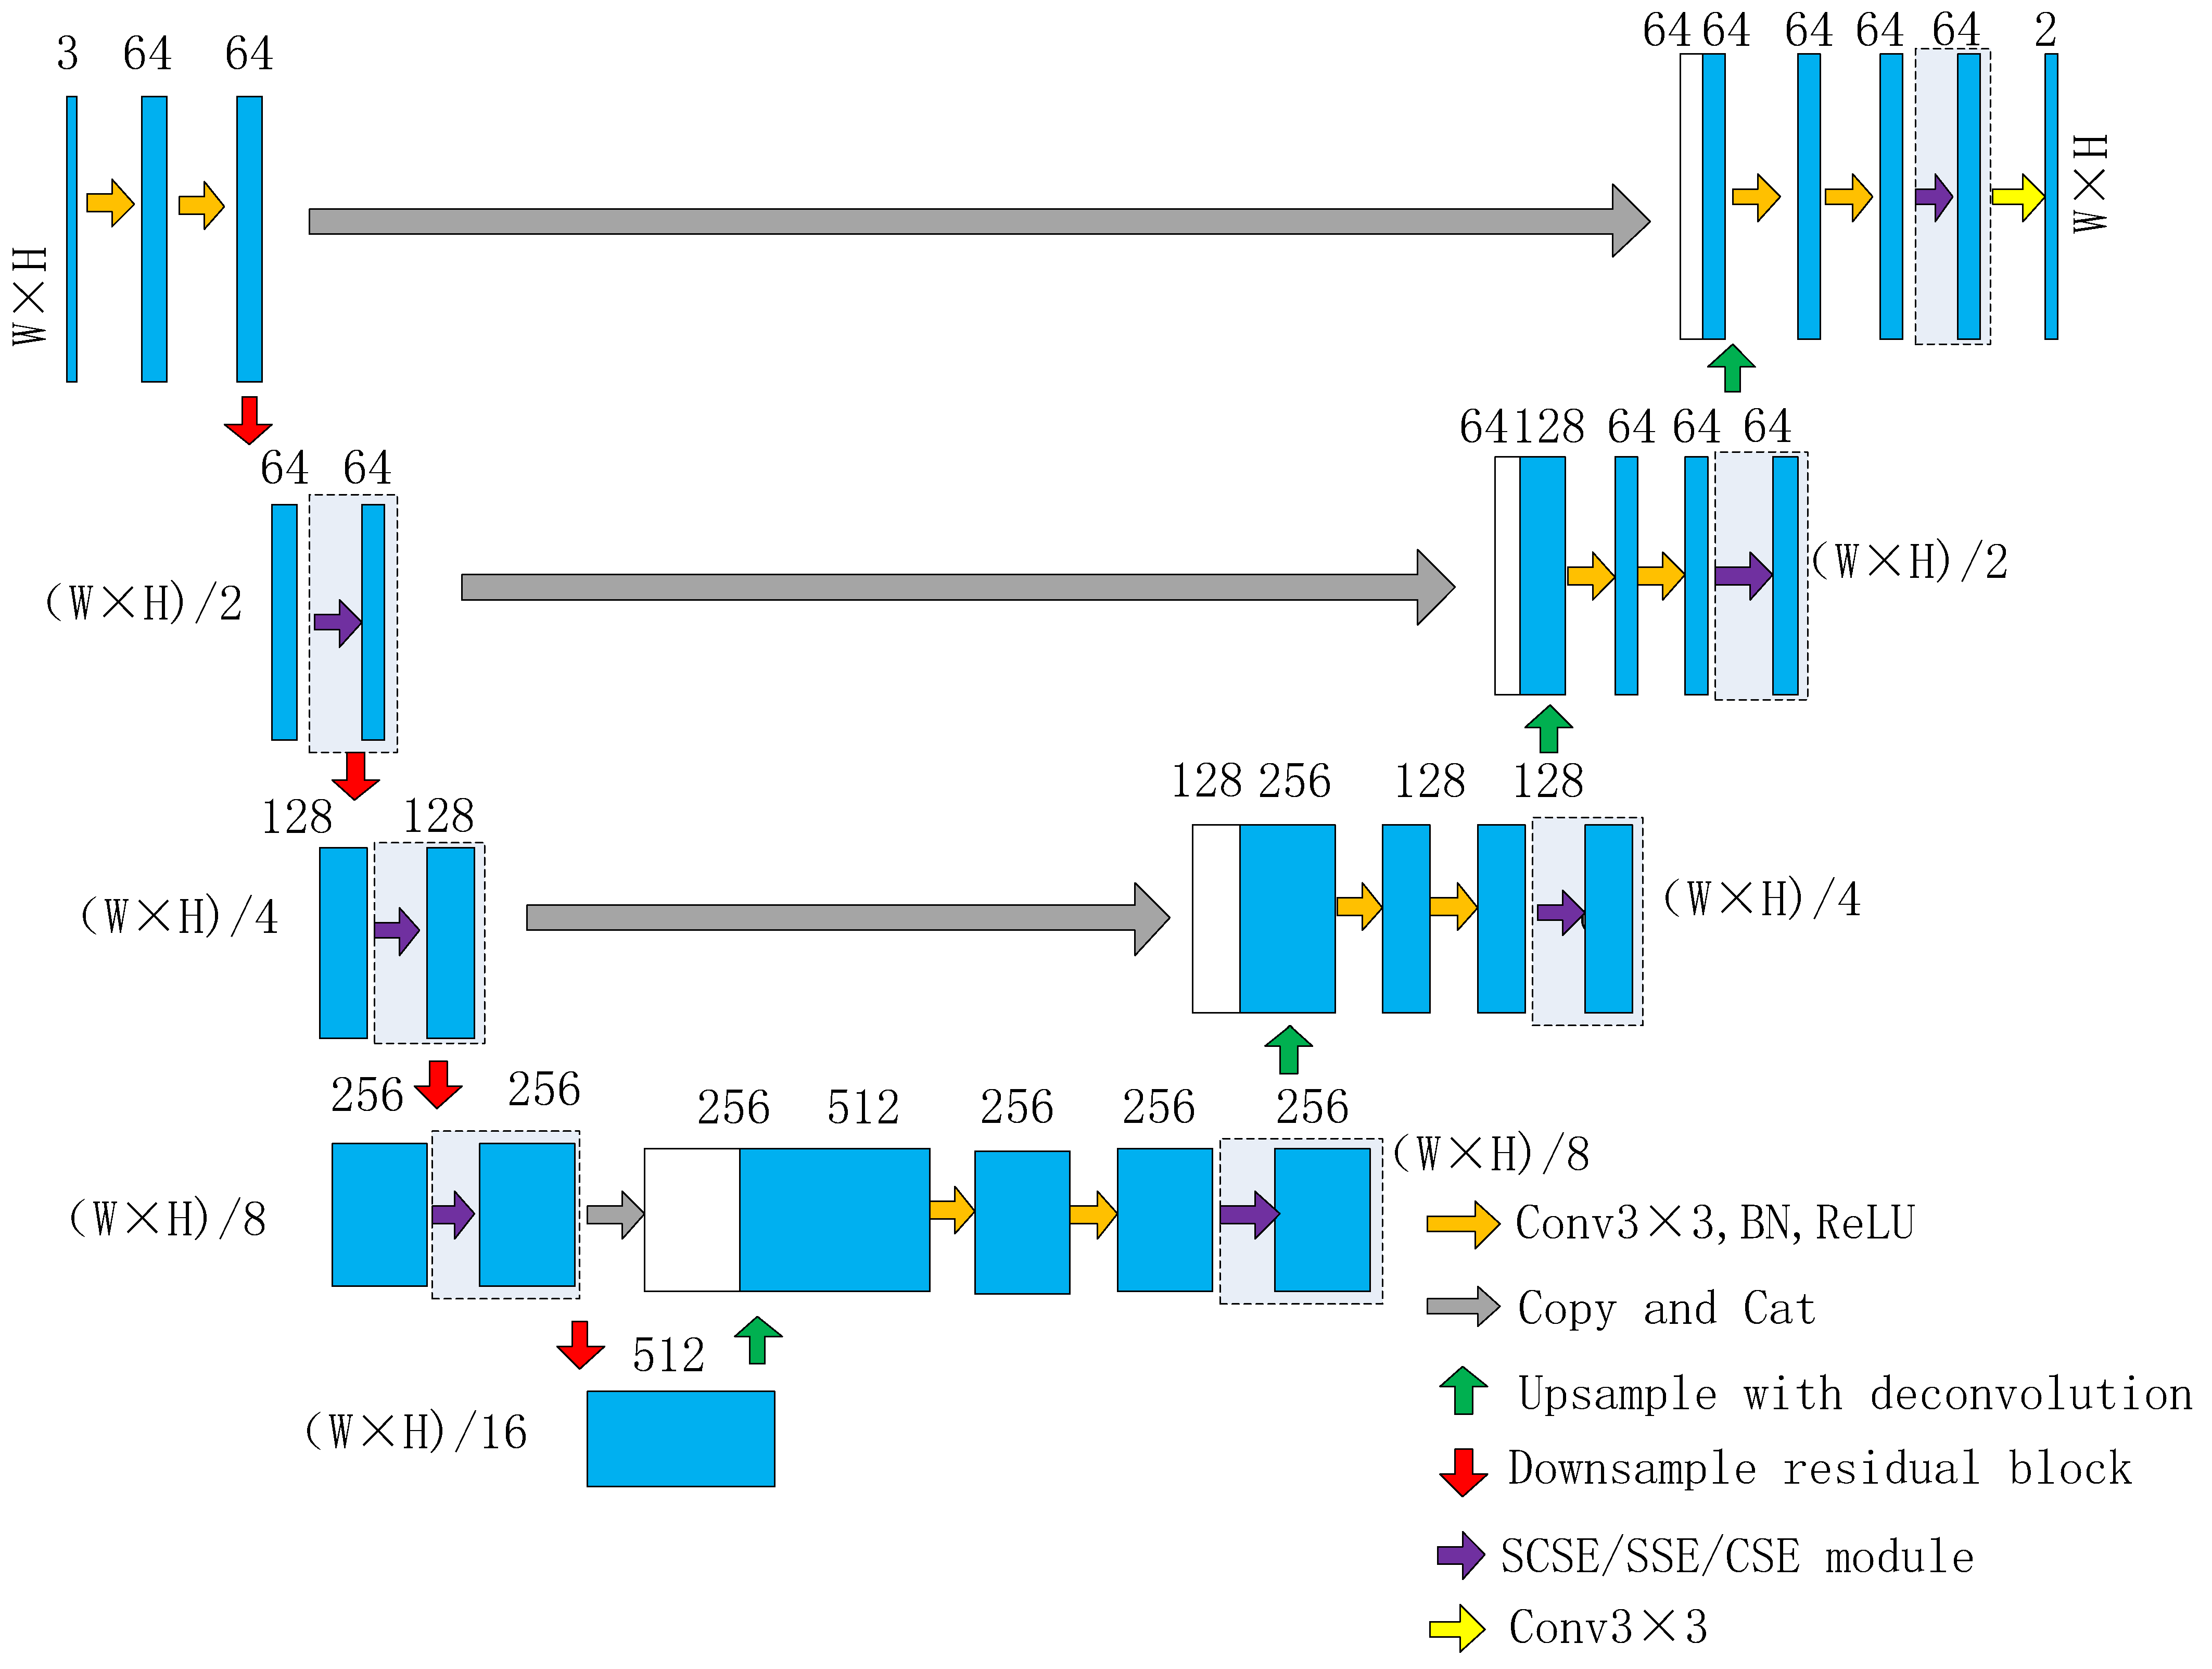
\includegraphics{../resources/u-net-architecture.png}
\caption{U-Net}
\end{figure}

    \hypertarget{fcn-fully-convolutional-network}{%
\subsubsection{FCN (Fully Convolutional
Network)}\label{fcn-fully-convolutional-network}}

FCN - это сверточная нейронная сеть, разработанная специально для задачи
семантической сегментации изображений.

\hypertarget{ux43eux441ux43dux43eux432ux43dux44bux435-ux445ux430ux440ux430ux43aux442ux435ux440ux438ux441ux442ux438ux43aux438}{%
\paragraph{Основные
характеристики:}\label{ux43eux441ux43dux43eux432ux43dux44bux435-ux445ux430ux440ux430ux43aux442ux435ux440ux438ux441ux442ux438ux43aux438}}

\begin{enumerate}
\def\labelenumi{\arabic{enumi}.}
\tightlist
\item
  \textbf{Сверточные слои:} Весь путь архитектуры FCN состоит из
  сверточных слоев. Отсутствие полносвязанных слоев позволяет работать с
  изображениями разных размеров и выполнять операции на пиксельном
  уровне.
\item
  \textbf{Сквозные соединения (Skip Connections):} Чтобы учесть детали
  объектов на разных масштабах, FCN использует сквозные соединения. Эти
  соединения передают информацию из слоев пути свертки к соответствующим
  слоям декодирования.
\item
  \textbf{Апсемплинг:} Для восстановления пространственной информации
  после сверточных операций уменьшения размера, в FCN используются
  операции апсемплинга. Обратные операции пулинга (unpooling) или
  операции деконволюции используются для восстановления размера
  изображения.
\item
  \textbf{Softmax слой:} В конце архитектуры применяется Softmax слой,
  который представляет вероятности для каждого пикселя относительно
  различных классов. Это позволяет получить карту сегментации, на
  которой каждому пикселю присваивается класс.
\end{enumerate}

\begin{figure}
\centering
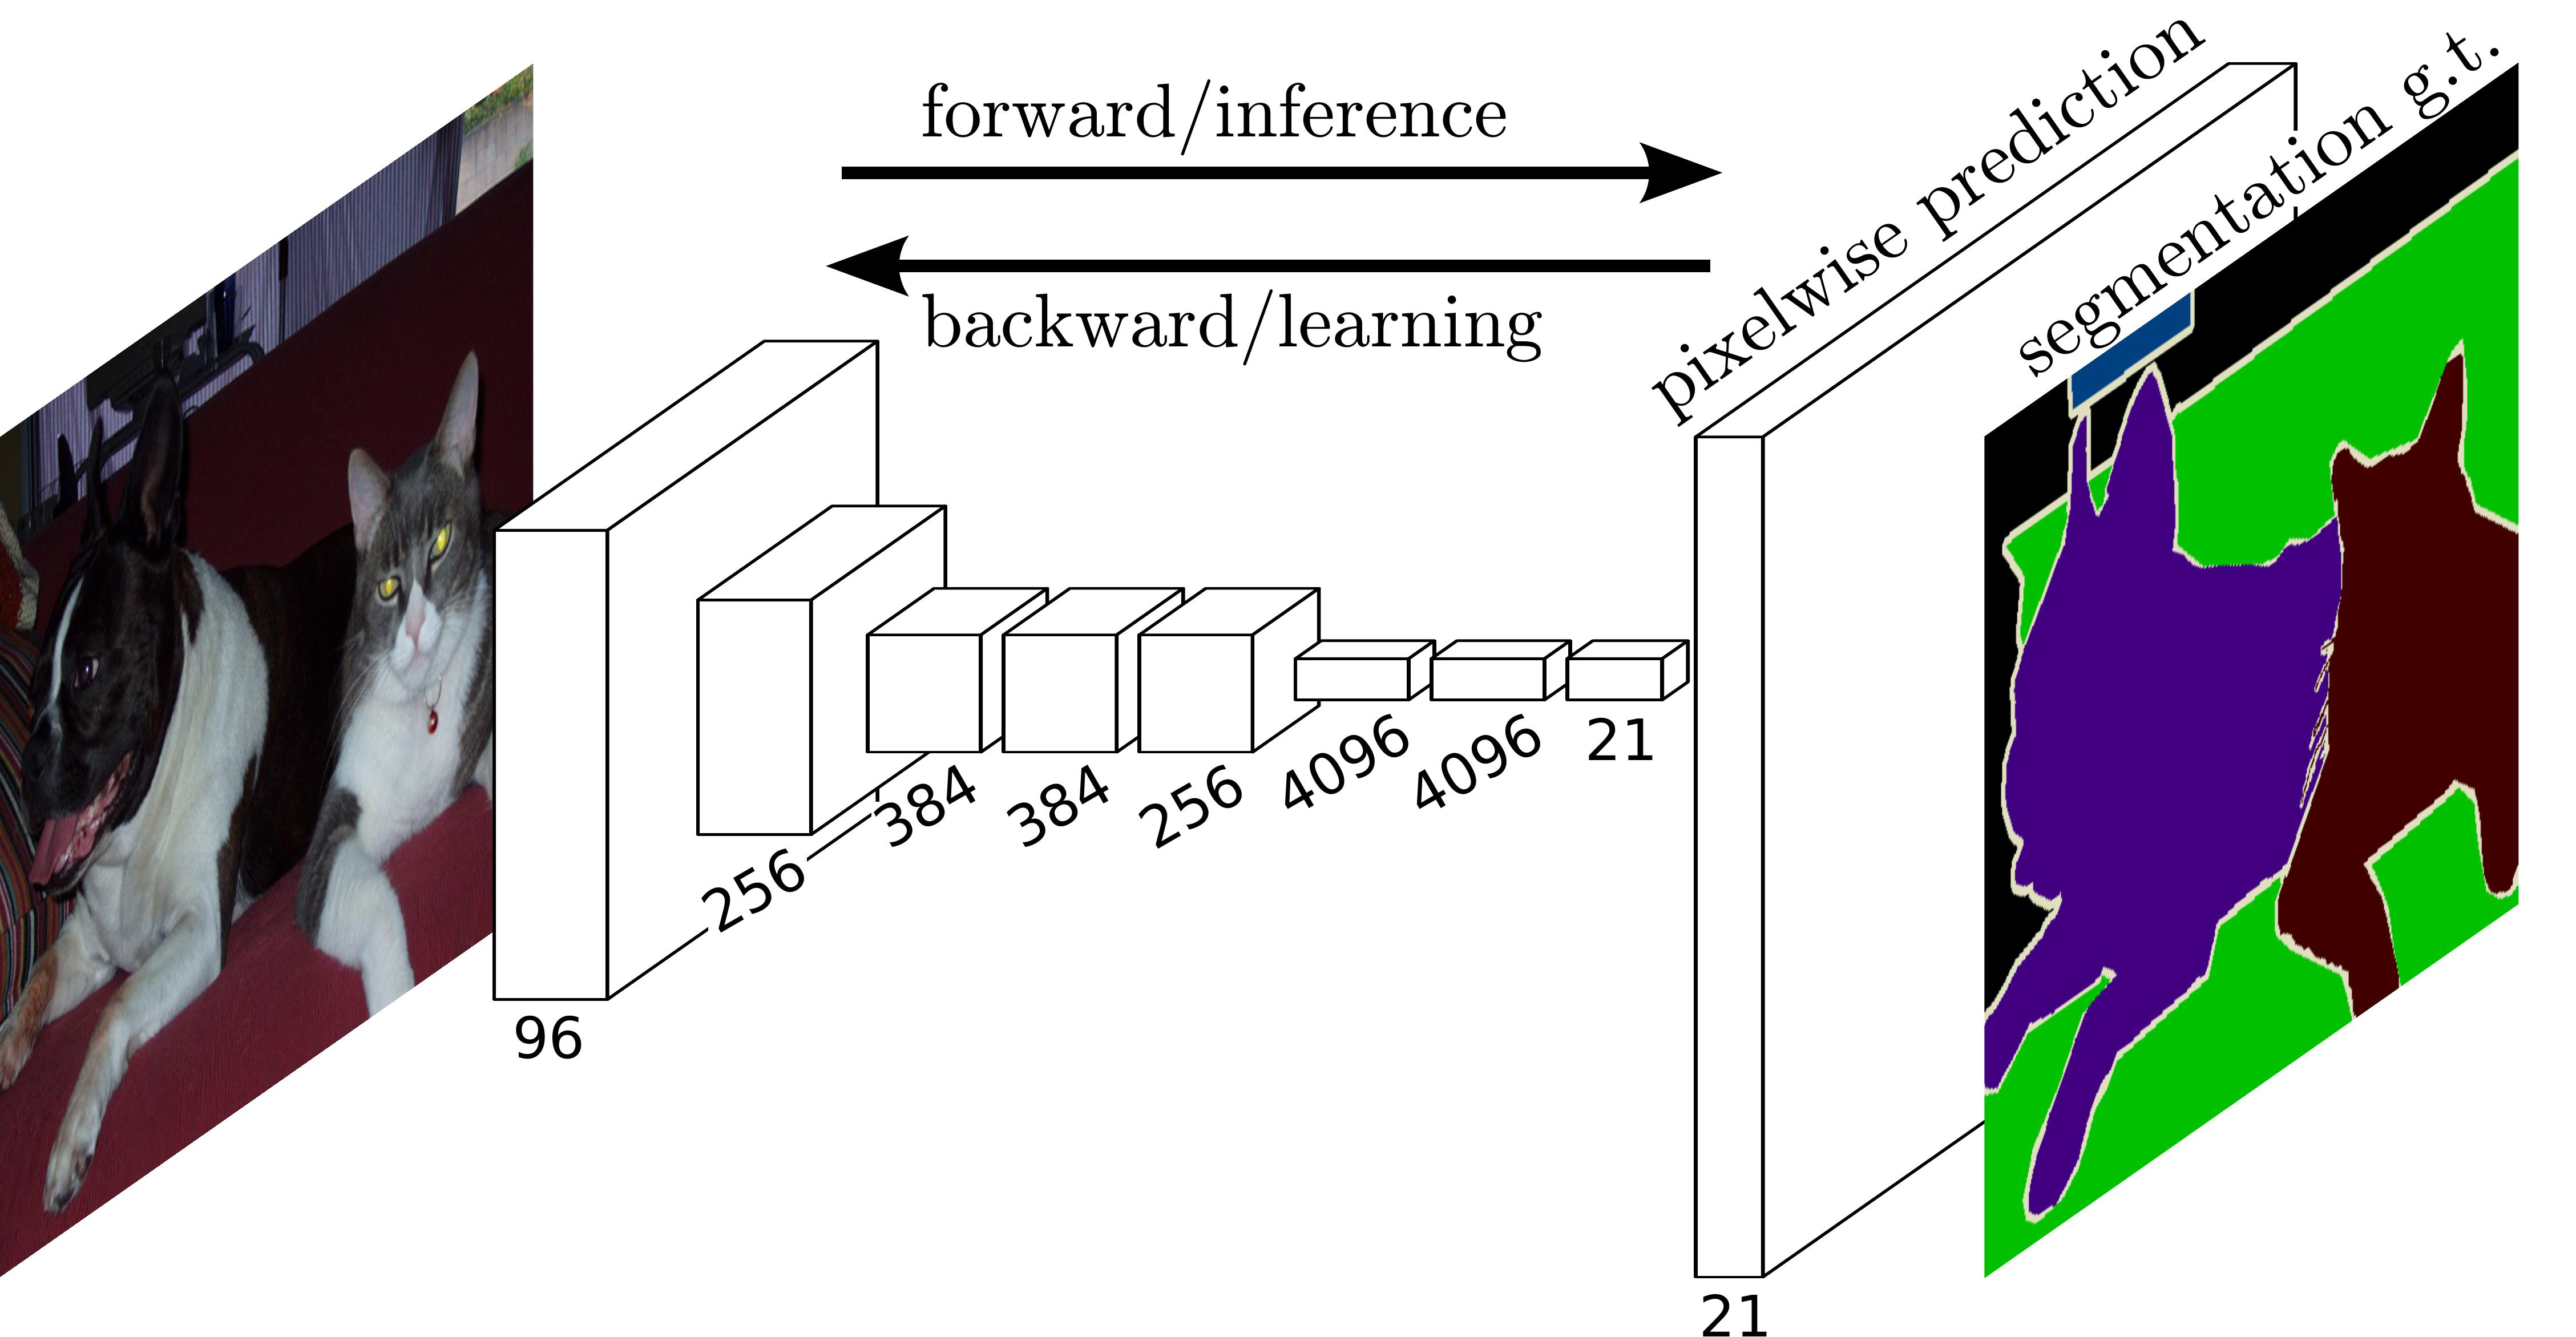
\includegraphics{../resources/fcn-architecture.jpg}
\caption{FCN}
\end{figure}

    \hypertarget{deeplab}{%
\subsubsection{Deeplab}\label{deeplab}}

DeepLab --- это архитектура семантической сегментации. Сначала входное
изображение проходит через сеть с использованием расширенных свёрток.
Затем выходные данные сети билинейно интерполируются и проходят через
полносвязный CRF для точной настройки результата, который мы получаем
для окончательных прогнозов.

\hypertarget{ux43eux441ux43dux43eux432ux43dux44bux435-ux445ux430ux440ux430ux43aux442ux435ux440ux438ux441ux442ux438ux43aux438}{%
\paragraph{Основные
характеристики:}\label{ux43eux441ux43dux43eux432ux43dux44bux435-ux445ux430ux440ux430ux43aux442ux435ux440ux438ux441ux442ux438ux43aux438}}

\begin{enumerate}
\def\labelenumi{\arabic{enumi}.}
\tightlist
\item
  \textbf{Ассоциативная CRF модель:} Одной из ключевых особенностей
  DeepLab является использование ассоциативной CRF (Conditional Random
  Field) модели для улучшения качества границ объектов. Эта модель
  обрабатывает карту сегментации и сглаживает границы между классами.
\item
  \textbf{Атрибутная декодирование:} DeepLab использует операцию
  декодирования для восстановления размера изображения и извлечения
  более детальной информации. Операция атрибутного декодирования
  позволяет извлекать более высокоуровневые признаки.
\item
  \textbf{Сверточные слои с большим шагом:} В архитектуре DeepLab
  применяются сверточные слои с большим шагом (dilated convolution), что
  позволяет увеличить приемное поле без потери пространственной
  разрешимости. Это помогает извлечь больше контекста.
\item
  \textbf{Использование предобученных моделей:} DeepLab может
  использовать предобученные модели, такие как ResNet, как основу для
  своей архитектуры. Это позволяет использовать предварительно обученные
  признаки и ускоряет процесс обучения.
\item
  \textbf{Multiscale аппроксимация:} Для учета объектов разных размеров
  DeepLab использует multiscale аппроксимацию, сочетая выходы разных
  слоев с разными масштабами. Это помогает достичь хорошей
  многомасштабной сегментации.
\end{enumerate}

Архитектура DeepLab эффективно обеспечивает высокую точность сегментации
объектов, а также устраняет артефакты и сглаживает границы. Её
способность обрабатывать детали делает её подходящей для задач,
требующих высокой степени точности.

\begin{figure}
\centering
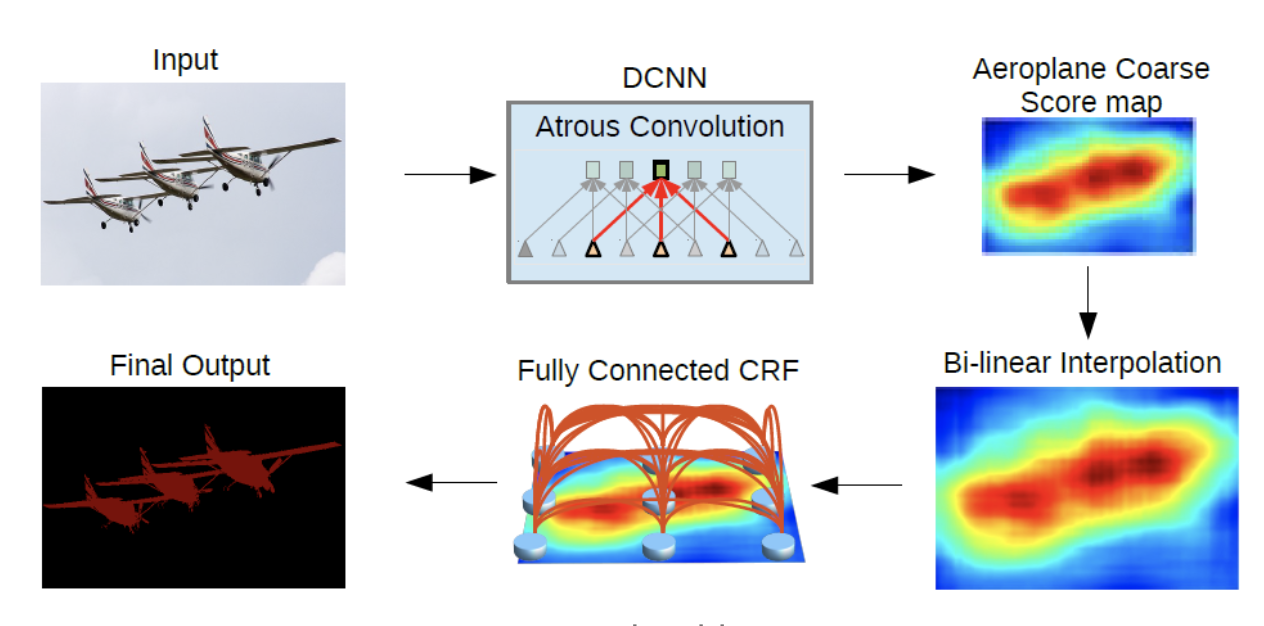
\includegraphics{../resources/deeplab-architecture.png}
\caption{Deeplab}
\end{figure}

    \hypertarget{fpn-feature-pyramid-network}{%
\subsubsection{FPN (Feature Pyramid
Network)}\label{fpn-feature-pyramid-network}}

Архитектура FPN разработана для улучшения разномасштабной обработки
изображений в сверточных нейронных сетях. Она позволяет моделям
эффективно работать с объектами разных размеров, обеспечивая
одновременно детализацию и контекст на разных уровнях масштаба.

\hypertarget{ux43eux441ux43dux43eux432ux43dux44bux435-ux445ux430ux440ux430ux43aux442ux435ux440ux438ux441ux442ux438ux43aux438}{%
\paragraph{Основные
характеристики:}\label{ux43eux441ux43dux43eux432ux43dux44bux435-ux445ux430ux440ux430ux43aux442ux435ux440ux438ux441ux442ux438ux43aux438}}

\begin{enumerate}
\def\labelenumi{\arabic{enumi}.}
\tightlist
\item
  \textbf{Encoder}: Как и в U-Net архитектуре в начале идет путь
  свертки. В качестве энкодера может использоваться ResNet архитектура.
\item
  \textbf{Пирамида признаков:} Особенностью FPN является пирамида
  признаков, которая объединяет признаки с разных уровней свертки. Это
  позволяет модели улавливать контекст и детали разных размеров.
\item
  \textbf{Сквозные связи:} FPN также использует сквозные связи для
  передачи информации из энкодера в FCN блоки напрямую.
\item
  \textbf{Сегментация:} В результате объединения признаков формируются
  карты признаков разных масштабов
\end{enumerate}

\begin{figure}
\centering
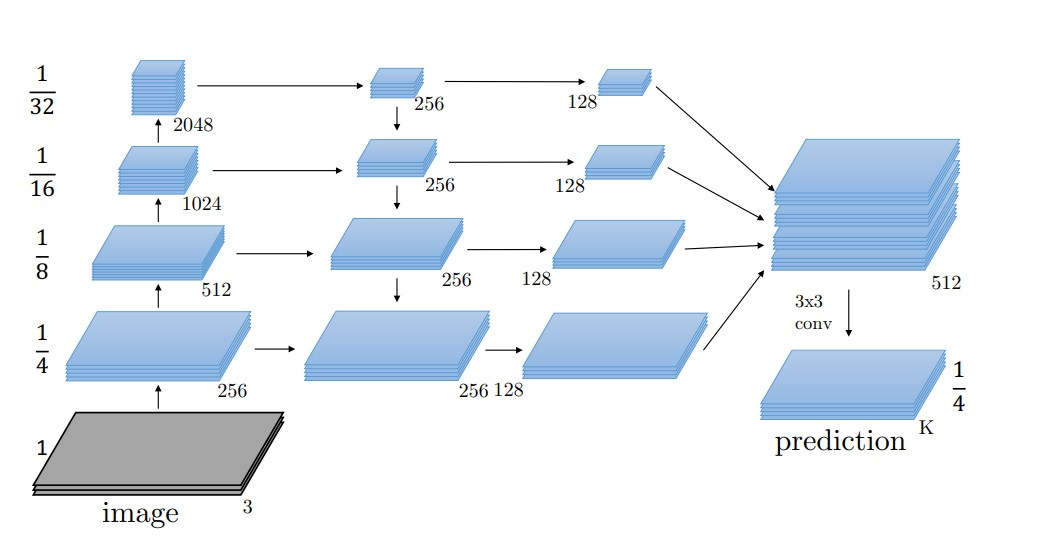
\includegraphics{../resources/fpn-architecture.jpg}
\caption{FCN}
\end{figure}

    \hypertarget{ux44dux43aux441ux43fux435ux440ux438ux43cux435ux43dux442ux430ux43bux44cux43dux43eux435-ux438ux441ux441ux43bux435ux434ux43eux432ux430ux43dux438ux435}{%
\subsection{Экспериментальное
исследование}\label{ux44dux43aux441ux43fux435ux440ux438ux43cux435ux43dux442ux430ux43bux44cux43dux43eux435-ux438ux441ux441ux43bux435ux434ux43eux432ux430ux43dux438ux435}}

    Для каждой архитектуры CNN (U-Net, FCN, DeepLab, FPN) были выбраны
соответствующие вариации моделей, учитывающие характерные особенности
каждой архитектуры. Обучение проходило на обучающем наборе данных
датасета ADE20K, который был разделен на обучающую и валидационную
выборки.

В процессе обучения нейронных сетей была замечена особенность, связанная
с функцией потерь DiceLoss. Данная функция потерь быстро достигала плато
при обучении, что затрудняло дальнейшее улучшение результатов модели. В
связи с этим, для повышения эффективности обучения и достижения лучших
результатов, было принято решение использовать комбинацию функций
потерь, CrossEntropyLoss и DiceLoss.

Для обучения были использованы оптимизатор Adam и механизм уменьшения
скорости обучения ReduceLROnPlateau, контролирующий метрику Dice score.

Для сохранения, анализа и визуального контроля результатов экспериментов
была выбрана платформа Weights and Biases (wandb). Эта платформа
предоставляет удобные инструменты для отслеживания процесса обучения,
анализа метрик и визуальной оценки результатов.

Результаты всех экспериментов доступны по адресу:
https://wandb.ai/losfantomaz/diploma

    Из проведенного экспериментального исследования стало явно видно, что
разные архитектуры сверточных нейронных сетей (CNN) имеют разные
скорости сходимости и качество сегментации в задаче обнаружения
проходимых поверхностей.

\hypertarget{ux441ux440ux430ux432ux43dux435ux43dux438ux435-ux430ux440ux445ux438ux442ux435ux43aux442ux443ux440-ux43fux43e-ux441ux43aux43eux440ux43eux441ux442ux438-ux441ux445ux43eux434ux438ux43cux43eux441ux442ux438}{%
\paragraph{Сравнение архитектур по скорости
сходимости}\label{ux441ux440ux430ux432ux43dux435ux43dux438ux435-ux430ux440ux445ux438ux442ux435ux43aux442ux443ux440-ux43fux43e-ux441ux43aux43eux440ux43eux441ux442ux438-ux441ux445ux43eux434ux438ux43cux43eux441ux442ux438}}

График функции потерь на этапе обучения позволяет сделать вывод, что
архитектуры Deeplab и FPN сходятся быстрее к оптимальным значениям
функции потерь по сравнению с U-Net и FCN.
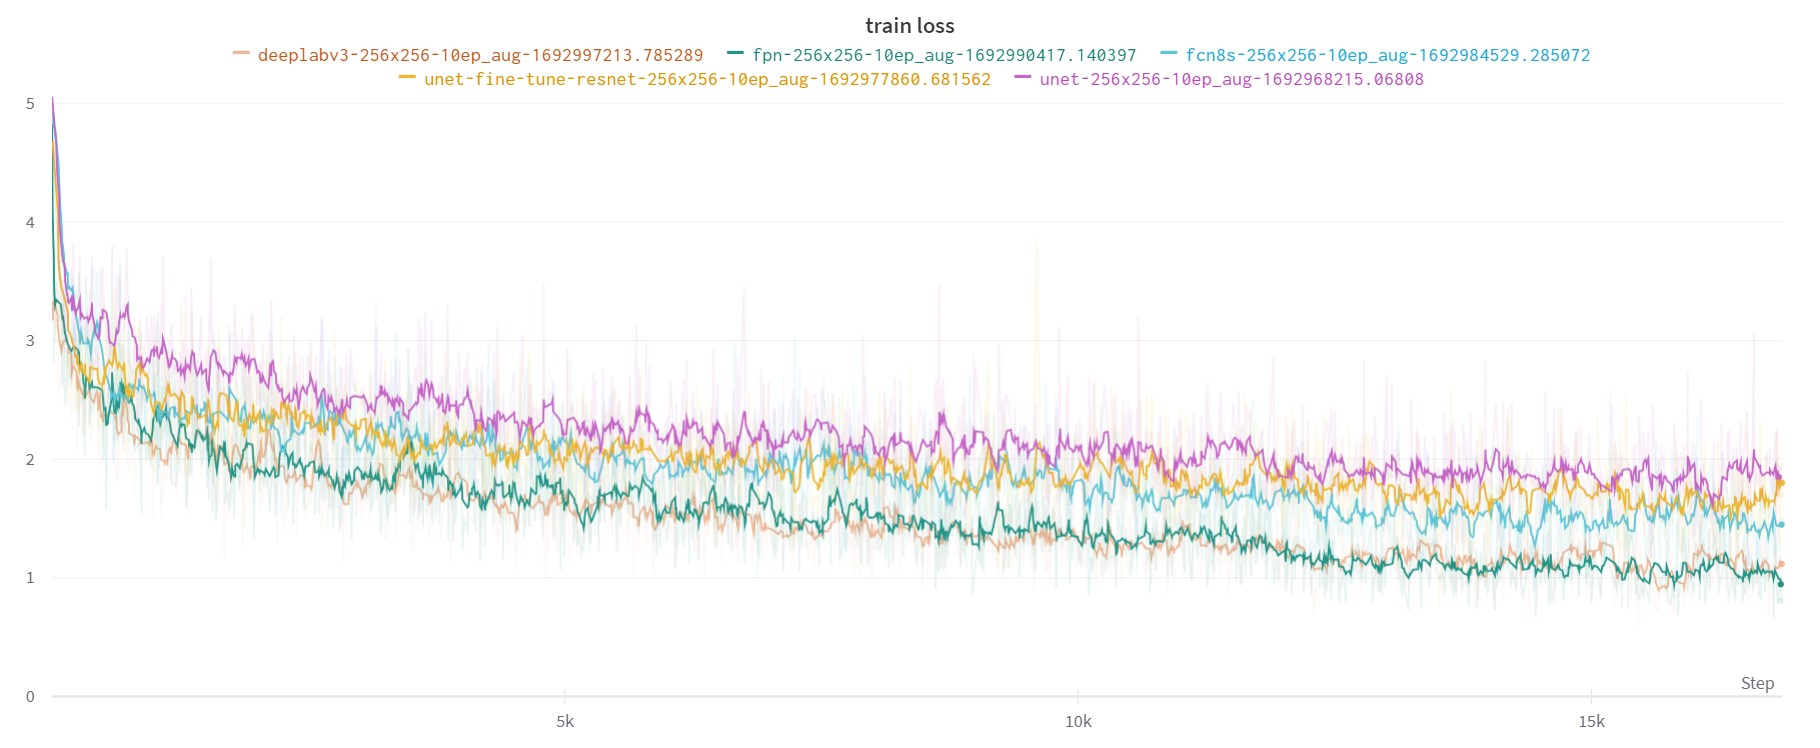
\includegraphics{../resources/train-loss.jpg}

\hypertarget{ux441ux440ux430ux432ux43dux435ux43dux438ux435-ux430ux440ux445ux438ux442ux435ux43aux442ux443ux440-ux43fux43e-ux43cux435ux442ux440ux438ux43aux430ux43c}{%
\paragraph{Сравнение архитектур по
метрикам}\label{ux441ux440ux430ux432ux43dux435ux43dux438ux435-ux430ux440ux445ux438ux442ux435ux43aux442ux443ux440-ux43fux43e-ux43cux435ux442ux440ux438ux43aux430ux43c}}

Анализ показателей метрик подтвердил, что Deeplab демонстрирует лучшие
результаты по всем метрикам: dice score, IoU и accuracy. Это говорит о
том, что Deeplab обеспечивает наиболее точную и качественную сегментацию
объектов на изображениях.

Архитектуры U-Net и FCN показали средние результаты по всем метрикам. В
сравнении с Deeplab и FPN, эти архитектуры отстают как по качеству
сегментации, так и по скорости сходимости. Это может быть связано с
менее сложной архитектурой и недостаточным учетом деталей изображения.

\begin{longtable}[]{@{}
  >{\raggedright\arraybackslash}p{(\columnwidth - 2\tabcolsep) * \real{0.5000}}
  >{\raggedright\arraybackslash}p{(\columnwidth - 2\tabcolsep) * \real{0.5000}}@{}}
\toprule\noalign{}
\begin{minipage}[b]{\linewidth}\raggedright
Dice score
\end{minipage} & \begin{minipage}[b]{\linewidth}\raggedright
IoU
\end{minipage} \\
\midrule\noalign{}
\endhead
\bottomrule\noalign{}
\endlastfoot
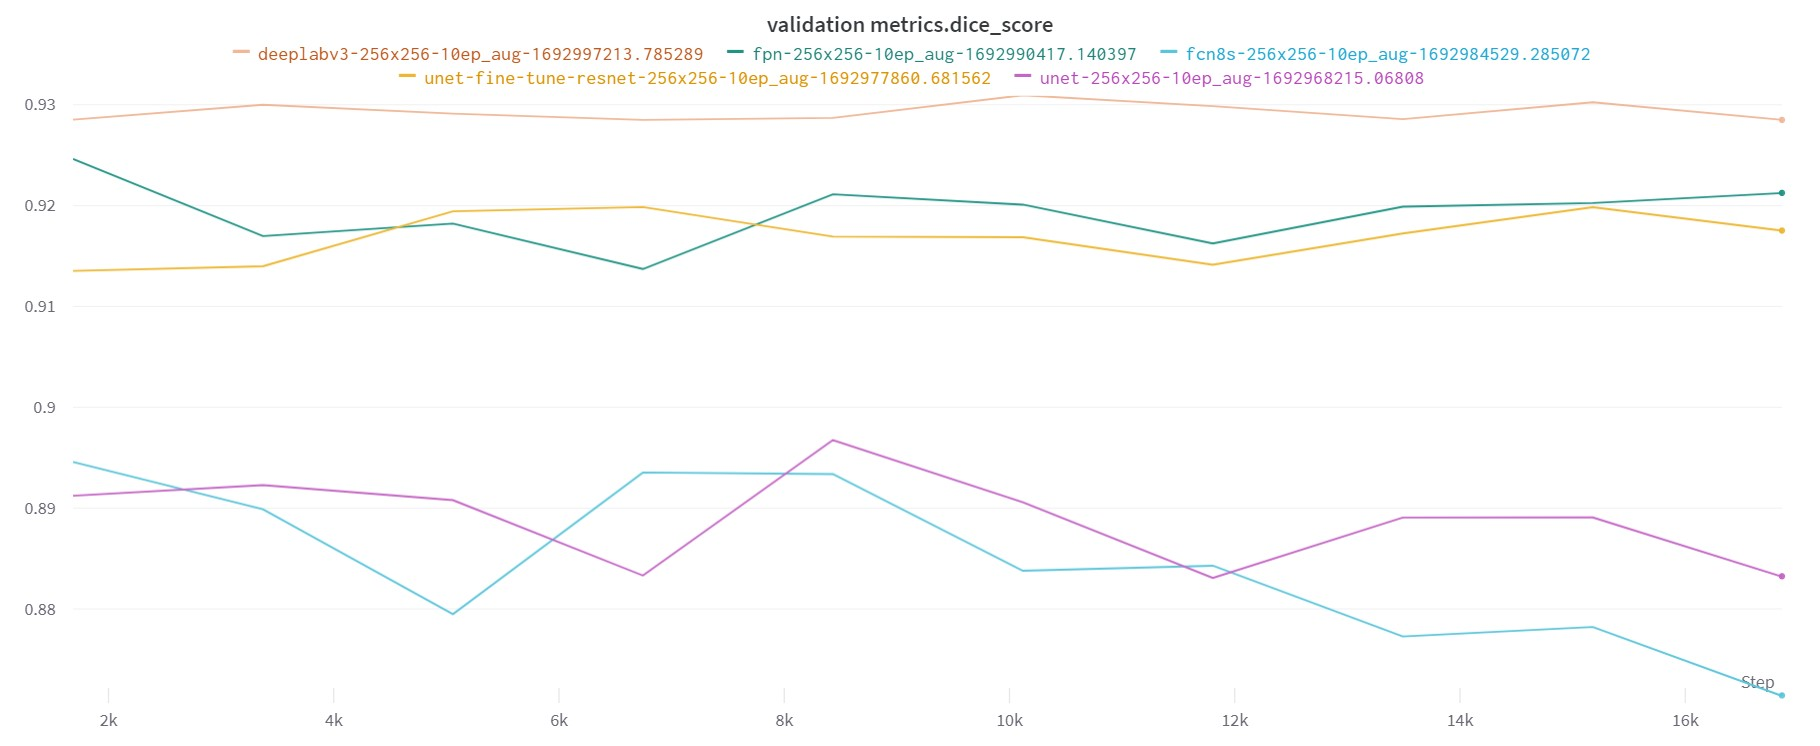
\includegraphics{../resources/dice-score-val.jpg} &
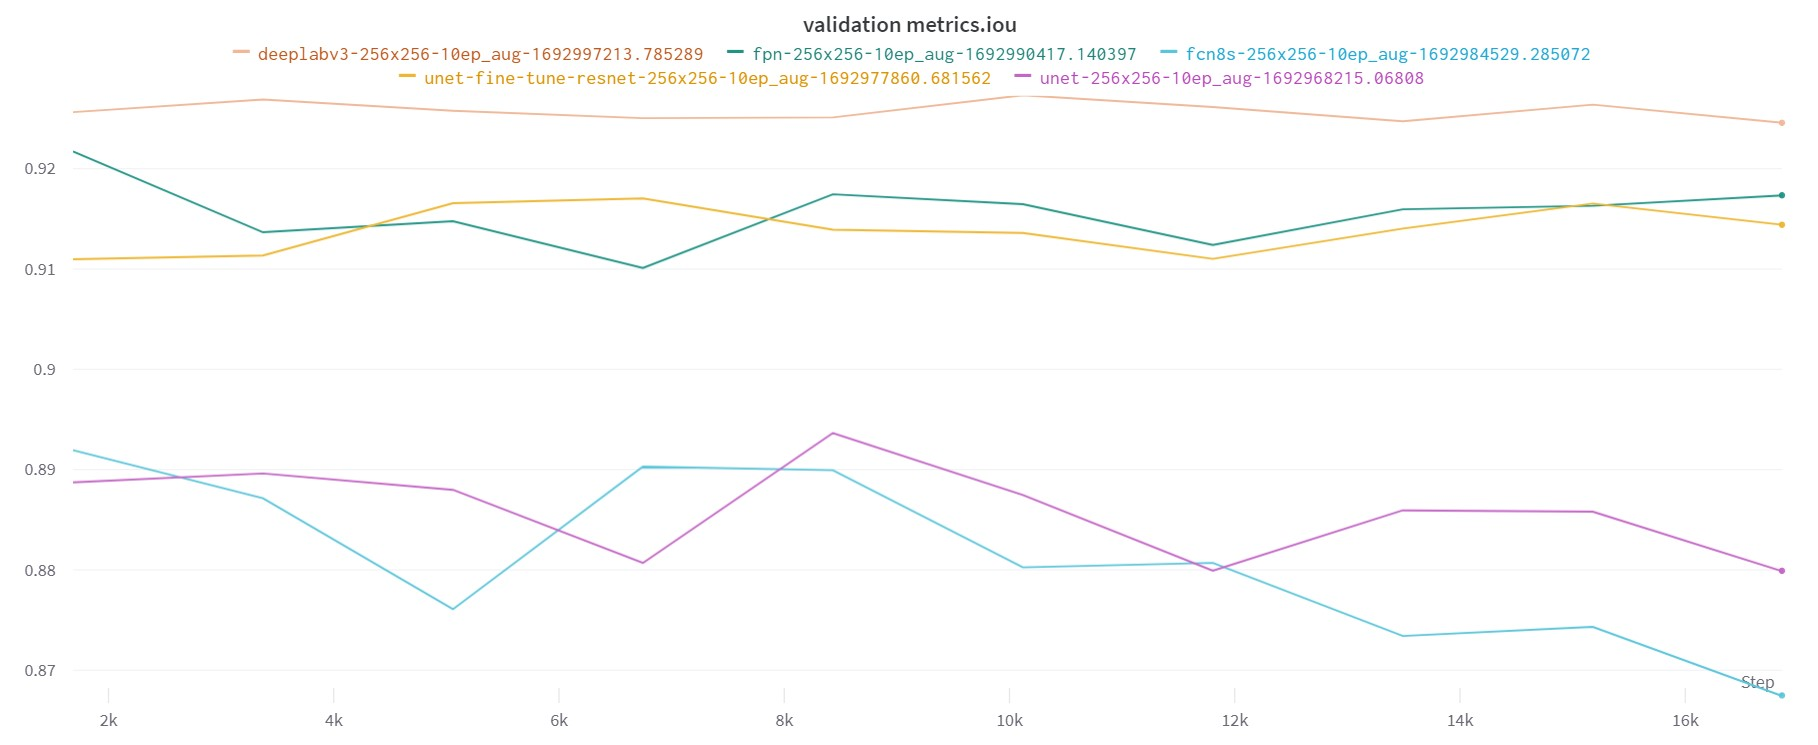
\includegraphics{../resources/iou-val.jpg} \\
\end{longtable}

    \hypertarget{ux440ux435ux437ux443ux43bux44cux442ux430ux442ux44b}{%
\paragraph{Результаты}\label{ux440ux435ux437ux443ux43bux44cux442ux430ux442ux44b}}

\begin{longtable}[]{@{}
  >{\raggedright\arraybackslash}p{(\columnwidth - 16\tabcolsep) * \real{0.1488}}
  >{\raggedright\arraybackslash}p{(\columnwidth - 16\tabcolsep) * \real{0.1653}}
  >{\raggedright\arraybackslash}p{(\columnwidth - 16\tabcolsep) * \real{0.0744}}
  >{\raggedright\arraybackslash}p{(\columnwidth - 16\tabcolsep) * \real{0.0661}}
  >{\raggedright\arraybackslash}p{(\columnwidth - 16\tabcolsep) * \real{0.0909}}
  >{\raggedright\arraybackslash}p{(\columnwidth - 16\tabcolsep) * \real{0.0992}}
  >{\raggedright\arraybackslash}p{(\columnwidth - 16\tabcolsep) * \real{0.0661}}
  >{\raggedright\arraybackslash}p{(\columnwidth - 16\tabcolsep) * \real{0.0992}}
  >{\raggedright\arraybackslash}p{(\columnwidth - 16\tabcolsep) * \real{0.1901}}@{}}
\toprule\noalign{}
\begin{minipage}[b]{\linewidth}\raggedright
Название модели
\end{minipage} & \begin{minipage}[b]{\linewidth}\raggedright
Размер изображения
\end{minipage} & \begin{minipage}[b]{\linewidth}\raggedright
mIoU
\end{minipage} & \begin{minipage}[b]{\linewidth}\raggedright
Dice
\end{minipage} & \begin{minipage}[b]{\linewidth}\raggedright
Accuracy
\end{minipage} & \begin{minipage}[b]{\linewidth}\raggedright
Precision
\end{minipage} & \begin{minipage}[b]{\linewidth}\raggedright
Recall
\end{minipage} & \begin{minipage}[b]{\linewidth}\raggedright
Train loss
\end{minipage} & \begin{minipage}[b]{\linewidth}\raggedright
Количество параметров
\end{minipage} \\
\midrule\noalign{}
\endhead
\bottomrule\noalign{}
\endlastfoot
U-Net & 256x256 & 0.8799 & 0.8832 & 0.9934 & 0.914 & 0.9555 & 2.52 &
31M \\
U-Net fine-tuned & 256x256 & 0.9144 & 0.9175 & 0.994 & 0.9507 & 0.956 &
3.749 & 24M \\
FCN & 256x256 & 0.8675 & 0.8714 & 0.9945 & 0.8966 & 0.9595 & 1.382 &
18.7M \\
FPN & 256x256 & 0.9174 & 0.9213 & 0.9951 & 0.9477 & 0.961 & 0.8848 &
23M \\
DeeplabV3 & 256x256 & 0.9246 & 0.9285 & 0.995 & 0.9557 & 0.961 & 1.269 &
26M \\
\end{longtable}

    \hypertarget{ux432ux44bux432ux43eux434ux44b}{%
\subsection{Выводы}\label{ux432ux44bux432ux43eux434ux44b}}

Исследование показало, что выбор функции потерь является важным фактором
при обучении нейронных сетей для семантической сегментации изображений.
Подход с использованием комбинированной функции потерь, CrossEntropyLoss
и DiceLoss, позволил улучшить качество сегментации. Однако, возможно,
подбор другой функции потерь, также может привести к дополнительным
улучшениям результатов. Например, функции потерь, ориентированные на
борьбу с дисбалансом классов (Focal Loss, Lovasz Softmax Loss), могут
быть рассмотрены для дальнейшего исследования.

Важным аспектом в разработке беспилотных систем и робототехнических
приложений является комплексное использование различных методов и
технологий. Нейронные сети могут быть успешно интегрированы с другими
методами, такими как определение расстояний с помощью дальномеров и
лидаров. Например, данные о расстояниях до препятствий, полученные с
дальномеров, могут быть использованы в качестве дополнительных признаков
для обучения нейронных сетей. Это позволит создать комплексную систему,
способную более точно сегментировать поверхности.

Такой подход позволяет объединить преимущества разных методов и улучшить
общую производительность системы. Комбинирование нейронных сетей с
дополнительными датчиками и алгоритмами распознавания окружающей среды
может обеспечить более надежное и точное решение задачи обнаружения
препятствий и определения проходимых путей в реальных условиях.

    \hypertarget{ux438ux441ux442ux43eux447ux43dux438ux43aux438}{%
\subsection{Источники:}\label{ux438ux441ux442ux43eux447ux43dux438ux43aux438}}

\begin{enumerate}
\def\labelenumi{\arabic{enumi}.}
\tightlist
\item
  https://arxiv.org/abs/2209.06078
\item
  Olaf Ronneberger, Philipp Fischer, and Thomas Brox. U-Net:
  Convolutional Networks for Biomedical Image Segmentation.
  https://arxiv.org/pdf/1505.04597.pdf
\item
  Jonathan Long, Evan Shelhamer, Trevor Darrell. Fully Convolutional
  Networks for Semantic Segmentation.
  https://arxiv.org/pdf/1411.4038.pdf
\item
  Alexander Kirillov, Kaiming He, Ross Girshick, Piotr Dollár. A Unified
  Architecture for Instance and Semantic Segmentation.
  http://presentations.cocodataset.org/COCO17-Stuff-FAIR.pdf
\item
  https://arxiv.org/pdf/1706.05587.pdf
\item
  http://sceneparsing.csail.mit.edu/ ADE20K датасет
\end{enumerate}

    


    % Add a bibliography block to the postdoc
    
    
    
\end{document}
